\documentclass[presentation]{beamer}
\usepackage[utf8]{inputenc}
\usepackage[T1]{fontenc}
\usepackage{graphicx}
\usepackage{grffile}
\usepackage{longtable}
\usepackage{wrapfig,epigraph}
\usepackage{rotating}
\usepackage[normalem]{ulem}
\usepackage{amsmath}
\usepackage{textcomp}
\usepackage{amssymb}
\usepackage{capt-of}
\usepackage{hyperref, tipa}
\let\pb\relax

\usepackage{tikz}
\usetikzlibrary{calc}
\makeatletter
\def\th@mystyle{%
    \normalfont % body font
    \setbeamercolor{block title example}{bg=red!5,fg=red!65!black}
    \setbeamercolor{block body example}{ bg=red!5,fg=black}
    \def\inserttheoremblockenv{exampleblock}
  }
\makeatother

\newcommand{\xto}[1]{\xrightarrow{#1}}
\newcommand{\xot}[1]{\xleftarrow{#1}}

\theoremstyle{mystyle}
	\newtheorem{df}{Definition}
	\newtheorem{oss}{Remark}
	\newtheorem{cor}{Corollary}
	\newtheorem{thm}{Theorem}
	\newtheorem{prop}{Proposition}
	\newtheorem{es}{Example}

\def\yo{y}
\def\shape{\text{\textesh}}
\def\thH{\widetilde{\clH}}
\def\disc{\textsc{disc}}
\def\codisc{\textsc{codisc}}

\usepackage{xparse}
\usepackage[all,2cell]{xy}\UseAllTwocells



\def\quadruple#1{%
	\ar@<12pt>@{^{(}->}[r]%
	\ar@{<-}@<4pt>[r]|{i^*_{#1}}%
	\ar@<-4pt>@{^{(}->}[r]|{i_{*,#1}}%
	\ar@<-12pt>@{<-}[r]%
 }

\ExplSyntaxOn
\NewDocumentCommand{\makeabbrev}{mmm}
 {
  \yoruk_makeabbrev:nnn { #1 } { #2 } { #3 }
 }

\cs_new_protected:Npn \yoruk_makeabbrev:nnn #1 #2 #3
 {
  \clist_map_inline:nn { #3 }
   {
    \cs_new_protected:cpn { #2 } { #1 { ##1 } }
   }
 }
\ExplSyntaxOff

\makeabbrev{\textbf}{bf#1}{
  a,b,c,d,e,g,h,i,j,k,l,m,n,o,p,q,r,t,u,v,w,x,y,z,%
  A,B,C,D,E,G,H,I,J,K,L,M,N,O,P,Q,R,T,U,V,W,X,Y,Z }
\makeabbrev{\boldsymbol}{bs#1}{%
    a,b,c,d,e,f,g,h,i,j,k,l,m,n,o,p,q,r,s,t,u,v,w,x,y,z,%
    A,B,C,D,E,F,G,H,I,J,K,L,M,N,O,P,Q,R,S,T,U,V,W,X,Y,Z }
\makeabbrev{\mathsf}{sf#1}{
  a,b,c,d,e,f,g,h,i,j,k,l,m,n,o,p,q,r,s,t,u,v,w,x,y,z,%
  A,B,C,D,E,F,G,H,I,J,K,L,M,N,O,P,Q,R,S,T,U,V,W,X,Y,Z }
\makeabbrev{\mathfrak}{fk#1}{
  a,b,c,d,e,f,g,h,j,k,i,l,m,n,o,p,q,r,s,t,u,v,w,x,y,z,%
  A,B,C,D,E,F,G,H,I,J,K,L,M,N,O,P,Q,R,S,T,U,V,W,X,Y,Z }
\makeabbrev{\mathcal}{cl#1}{
  A,B,C,D,E,F,G,H,I,J,K,L,M,N,O,P,Q,R,S,T,U,V,W,X,Y,Z }
\makeabbrev{\mathbb}{bb#1}{
  A,B,C,D,E,F,G,H,I,J,K,L,M,N,O,P,Q,R,S,T,U,V,W,X,Y,Z }

\newlength{\seplen}
\setlength{\seplen}{5pt}
\newlength{\sepwid}
\setlength{\sepwid}{.4pt}
\def\firstblank{\,\rule{\seplen}{\sepwid}\,}
\def\secondblank{\firstblank\llap{\raisebox{2pt}{\firstblank}}}
\def\To{\Rightarrow}

\def\Set{\underline{\text{Set}}}
\newcommand{\op}{\text{op}}

\setbeamertemplate{navigation symbols}{}
\usepackage{animate}

\newenvironment{variableblock}[3]{%
  \setbeamercolor{block body}{#2}
  \setbeamercolor{block title}{#3}
  \begin{block}{#1}}{\end{block}}

\newenvironment{myblock}[1]{%
	\begin{variableblock}{#1}{bg=blue!10, fg=black}{bg=blue!10, fg=blue}%
	}{%
	\end{variableblock}%
	}


\usetheme{metropolis}
\author{Fosco Loregian \\[3pt] 
\includegraphics[scale=1.5]{logo.pdf}}
\date{\today}
\title{Cohesion in Rome}
\begin{document}

\maketitle
\begin{frame}{Outline}
	\linespread{.66}
	\epigraph{
    \tiny [\dots\unkern] vi el Aleph, desde todos los puntos, vi en el Aleph la tierra, y en la tierra otra vez el Aleph y en el Aleph la tierra, vi mi cara y mis vísceras, vi tu cara, y sentí vértigo y lloré\dots%
    }{JLB}
	\linespread{1}
	Topos theory is a cornerstone of category theory linking together algebra, geometry and logic.

  \onslide<2->
	Simply said, in each topos it is possible to re-enact the totality of known Mathematics; today we focus on
	\begin{itemize}
		\item<+-> Logic (better said, a fragment of \alert{dependent type theory})
		\item<+-> Differential geometry
		\item<+-> Algebraic topology
		\item<+-> \dots
	\end{itemize}
\end{frame}
\begin{frame}[label={sec:orgd0201f8}]{Definizione di fascio su uno spazio}
	\begin{block}{}
		Let $(X,\tau)$ be a topological space; a \emph{sheaf on $X$} is a functor $F : \tau^\op\to \Set$ such that for every $U\in\tau$ and every covering $\{U_i\}$ of $U$ one has
		\begin{itemize}
			\item<+-> if $s, t\in FU$ are such that $s|_i = t|_i$ in $FU_i$ for every $i\in I$, then $s=t$ in $FU$.
			\item<+-> if $s_i\in FU_i$ is a family of elements such that $s_i|_{ij} = s_j|_{ij}$, then there exists a $s\in FU$ such that $s|_i = s_i$.\footnote{We denote $s|_i$ the image of $s\in FU$ under the nmeless map $FU\to FU_i$ induced by the inclusion $U_i\subseteq U$.}
		\end{itemize}
	\end{block}
\end{frame}
\begin{frame}{Examples of sheaves}
	Every construction in Mathematics that exhibits a local character is a sheaf:
	\begin{itemize}
		\item<+-> sending $U\mapsto CU$, continuous functions with domain $U$ (similarly, differentiable, $C^\infty$, $C^\omega$, holomorphic\dots)
		\item<+-> sending $U\mapsto \Omega^pU$, differential forms supported on $U$ (similarly: distributions, test functions\dots)
		\item<+-> \dots sending $U\mapsto \{f : U \to \mathbb R \mid f \text{ has property $P$ locally}\}$ for some $P$.
	\end{itemize}
	\onslide<+->
	Every construction that does involve global properties, is not a sheaf:
	\begin{itemize}
		\item<+-> sending $U\mapsto \{\text{bounded functions } f : U \to \mathbb R\}$
		\item<+-> sending $U\mapsto \{L^1\text{ functions } f : U \to \mathbb R\}$
		\item<+-> \dots
	\end{itemize}
\end{frame}
\begin{frame}[label={sec:org4e45118}]{Definizione di topa di Groto}
	A \emph{sieve} on an object $X$ of a category $\clC$ is a subobject $S$ of the hom functor $\yo X = \clC(\firstblank,X)$;

	A \emph{Grothendieck topology} on a category amounts to the choice of a family of \emph{covering sieves} for every object $X\in\clC$; this family of sieves is chosen in such a way that
	\begin{itemize}
		\item if $S\To \yo X$ is a covering sieve and $f : Y \to X$ is a morphism of $\clC$, then the morphism $f^* S \To Y$ obtained in the pullback
		      \[\xymatrix{
				      f^*S \ar@{}[dr]|\lrcorner \ar[r]\ar[d]& S \ar[d]\\
				      Y \ar[r]_f & X
			      }\]
		      is again a covering sieve.
	\end{itemize}
\end{frame}
\begin{frame}
	\begin{itemize}
		\item Let $S \To yX$ be a covering sieve on $X$, and let $T$ be any sieve on $X$. If for each object $Y$ of $\clC$ and each arrow $f : Y \to X$ in $SY$ the pullback sieve $f^*T$ is a covering sieve on $Y$, then $T$ is a covering sieve on $X$.
		\item the identity $1 : \yo X\To \yo X$ is a covering sieve.
	\end{itemize}
	\alert{\tiny
		\begin{itemize}
			\item<+-> if $\{U_i\}$ covers $U$, then for every $V\subseteq U$ $V\cap U_i$ covers $V$;
			\item<+-> if $\{U_i\}$ covers $U$ and $\{V_{ij}\}$ covers $U_i$, then $V_{ij}$ covers $U$;
			\item<+-> $\{U\}$ covers $U$.
		\end{itemize}
	}
	\onslide<+->
	A \alert{Grothendieck site} is a category with a Grothendieck topology, i.e. a function $j$ that assigns to every object a family of covering sieves.

	We denote a site as the pair $(\clC,j)$.
\end{frame}
\begin{frame}[label={sec:org9262f53}]{Definizione di fascio su un sito}
	\begin{block}{}
		A \emph{sheaf} on a small site $\clC$ is a functor $F : \clC^\op\to\Set$ such that for every covering sieve $R \to \yo U$ and every diagram
		\[\xymatrix{
				R \ar[r]^f\ar[d]_m & F \\
				\yo U\ar@{.>}[ur]
			}\]
		there is a unique dotted extension $\yo U \To F$ (by the Yoneda lemma, this consists of a unique element $s\in FU$, \textbf{exercise}).

		The full subcategory of sheaves on a site $(\clC,j)$ is denoted $\text{Sh}(\clC,j)$.
	\end{block}
\end{frame}
\begin{frame}[label={sec:org5bf1529}]{Cat dei fasci è riflessiva, Giraud}
	By general facts on locally presentable categories, the subcategory of sheaves on a site is reflective via a functor
	\[
		r : \textbf{Cat}(\clC^\op,\Set) \to \text{Sh}(\clC,j)
	\] called \emph{sheafification} of a presheaf $F : \clC^\op\to \Set$.

	\begin{block}{Historical note}
		\vspace{3pt}
		\scriptsize
		Grothendieck was the first to note that in every topos of sheaves the \alert{internal language} is sufficiently expressive to concoct \alert{higher-order logic} and he strived to advertise his intuitions to an audience of logicians.

		But it wasn't until Lawvere devised the notion of \alert{elementary topos} that the community agreed on the potential of this theory.
	\end{block}
\end{frame}
\begin{frame}[label={sec:org6a1b958}]{Definizione di topos elementare}
	\begin{block}{}
		An \emph{elementary topos} is a category $\clE$ that
		\begin{itemize}
			\item it has finite limits;% finitely complete (i.e. it admits finite products and equalizers, or a terminal object and pullbacks, or all limits of diagrams $D : \clJ \to \clE$ where $\clJ$ is a finite category);
			\item is cartesian closed;%, i.e. the functor $A\times\firstblank$ has a right adjoint $[A,\firstblank]$ for every object $A\in\clE$
			\item has a \emph{subobject classifier}, i.e. an object $\Omega\in\clE$ such that the functor $\text{Sub} : \clE^\op\to \Set$ sending $A$ into the set of isomorphism classes of monomorphisms $\begin{smallmatrix}{U}\\\downarrow\\{A}\end{smallmatrix}$ is representable by the object $\Omega$.
		\end{itemize}
	\end{block}
\end{frame}
\begin{frame}{Definizione di topos elementare}
	The natural bijection $\clE(A,\Omega)\cong\text{Sub}(A)$ is obtained pulling back the monomorphism $U\subseteq A$ along a \emph{universal arrow} $t : 1\to \Omega$, as in the diagram
	\[
		\vcenter{\xymatrix@!=3mm{
		U \ar@{}[dr]|\lrcorner \ar[r]\ar[d]_m & 1\ar[d]^t \\
		A \ar[r]_{\chi_m}& \Omega
		}}
	\]
	so, the bijection is induced by the maps
	\begin{itemize}
		\item $\chi_{-} : \left[\begin{smallmatrix}
					      U \\ \downarrow \\ A
				      \end{smallmatrix} \right]\mapsto \chi_m$ and
		\item $-\times_\Omega t : \chi_U \mapsto \chi_U \times_\Omega t$.
	\end{itemize}
\end{frame}
\begin{frame}[label={sec:orgb2a88e9}]{Groto = elem + locpres (finito)}
  These two seemingly disconnected definitions are in fact very similar to one another:
  \begin{itemize}
    \item Every Grothendieck topos is elementary;
    \item An elementary topos is Grothendieck if and only if it is a locally finitely presentable category.
  \end{itemize}
  [say more on Giraud theorem]
\end{frame}
\begin{frame}[label={sec:org0dca741}]{Logica e omotopia dei topos}
\end{frame}



\begin{frame}{What is cohesion}%{movie}
	Cohesion is the mutual attraction of molecules sticking together to form \emph{droplets}, caused by mild electrical attraction between them.
  \onslide<+->
  
  [here be image]
	% \begin{figure}[h!]
	% 	\centering
	% 	\animategraphics[loop,width=0.5\textwidth]{12}{materiale/cohesion-pngs/cohesion-}{0}{200}
	% 	%\includegraphics[width=0.5\textwidth]{example-image-b.png}
	% 	\caption{Droplets of mercury ``exhibiting cohesion''}
	% \end{figure}
\end{frame}
\begin{frame}{What is cohesion}%{movie}
	\onslide<+->
  Classes of geometric spaces exhibit similar coagulation properties, \onslide<+->similar to internal forces leading them to adhere and form \alert{coherent conglomerates}. \onslide<+->This behaviour is typical of \alert{smooth spaces}.% fundamental components of these spaces are these adherent ``droplets''.

	\medskip

	\onslide<+->\begin{variableblock}{Example}{bg=blue!10, fg=black}{bg=blue!10, fg=black}
		\alert{Smooth manifolds} can be probed via smooth open balls and every smooth space is a ``coherent conglomerate'' of \emph{cohesive pieces}.
	\end{variableblock}
	\vspace*{\fill}
	\onslide<+->\begin{variableblock}{Question}{bg=red!10, fg=black}{bg=red!10, fg=blue}
		Which formal axioms describe the mathematics behind this intuition? What is \emph{axiomatic cohesion}?
	\end{variableblock}

	\vspace*{\fill}
	Axioms to answer this question have been devised by Lawvere [Law1] (worthy reading, but quite mystical!).
\end{frame}
%
%
%
%
%
%
%
%
%
\begin{frame}{Desiderata}
	\onslide<+->
	We would like to operate in a \emph{category} (a \alert{topos}) of ``cohesive spaces'', such that
	\begin{itemize}
		\item<+-> there is a functor $\Pi \colon \clH \to \Set$ that sends every cohesive space $X\in\clH$ into its set of \alert{connected components}.
		\item<+-> Every set $S\in\Set$ can be regarded as a cohesive space in two complementary ways:
		      \begin{itemize}
			      \item<+-> \emph{discretely}, with a functor $\Set\to\clH$ that regards every singleton of $S$ as a cohesive droplet;
			      \item<+-> \emph{codiscretely}, with a functor $\Set\to\clH$ that regards the whole $S$ as an unseparable cohesive droplet.
		      \end{itemize}
		\item<+-> Discretely and codiscretely cohesive spaces embed  in $\clH$, with fully faithful functors: in that
		      \begin{gather*}
            \clH(\disc(S),\disc(T))\cong \Set(S,T) \\
			      \clH(\codisc(S),\codisc(T))\cong \Set(S,T) 
          \end{gather*}
	\end{itemize}
\end{frame}
%
%
%
%
%
%
%
%
%
\begin{frame}{Axiomatic cohesion}
	\onslide<+->
	An adjunction
	\[
		\alert{\Pi\dashv \disc\dashv\Gamma\dashv \codisc} :
		\xymatrix@C=3cm{
		\clH \ar@{}[r]|(.75)\perp
		\ar@{}@<10pt>[r]|(.75)\perp
		\ar@{}@<-10pt>[r]|(.75)\perp
		\ar@<15pt>[r]^{\Pi}
		\ar@<-5pt>[r]|\Gamma
		&
		\ar@<-5pt>[l]|{\disc}
		\ar@<15pt>[l]^{\codisc}
		\Set
		}
	\]
	\textbf{exhibits the cohesion of $\clH$ over $\Set$} if %is called a \alert{cohesive arrangement} or a \alert{cohesion}, if:
	\begin{itemize}
		\item<+-> $\disc$ and $\codisc$ are fully faithful;
		\item<+-> the leftmost adjoint $\Pi$ preserves finite products.
  \end{itemize}
  ($\Gamma$ ``forgets cohesion'': it sends a space to its underlying set of points)
	% \onslide<+->
	% \begin{block}{}
	% 	Host of nice properties follow from these astoundingly simple requests.
	% \end{block}
	% \onslide<+->\large $\clH$ is called a \emph{cohesive topos} or it is said that ``\alert{$\clH$ exhibits cohesion}''.
\end{frame}
%
%
%
%
%
%
%
%
%
\begin{frame}
	\onslide<+->
	\begin{block}{}
		\textbf{Formal fact.} Every quadruple of adjoints induces a triple of adjoints.
	\end{block}
	\onslide<+->
		\begin{itemize}
			% \item<+-> $\codisc$ is fully faithful as well;
			\item<+-> There is an adjoint triple of idempotent co/monads on $\clH$, induced by the cohesion:
			      \[
				      \alt<5>{
				      \xymatrix@C=3cm{
				      \clH
				      \ar@{}@<8pt>[r]|(.75)\perp
				      \ar@{}@<-8pt>[r]|(.75)\perp
				      \ar@[red]@<15pt>[r]^{\color{red}\Pi}
				      \ar@[blue]@{<-}[r]|{\color{blue}\disc}
				      \ar@[green]@<-15pt>[r]_{\color{green}\Gamma}
				      &
				      \Set
				      \ar@{}@<8pt>[r]|(.75)\perp
				      \ar@{}@<-8pt>[r]|(.75)\perp
				      \ar@[red]@<15pt>[r]^{\color{red}\disc}
				      \ar@[blue]@{<-}[r]|{\color{blue}\Gamma}
				      \ar@[green]@<-15pt>[r]_{\color{green}\codisc}
				      &
				      \clH}
				      }{\xymatrix@C=3cm{
				      \clH
				      \ar@{}@<8pt>[r]|(.75)\perp
				      \ar@{}@<-8pt>[r]|(.75)\perp
				      \ar@<15pt>[r]^\Pi
				      \ar@{<-}[r]|\disc
				      \ar@<-15pt>[r]_\Gamma &
				      \Set
				      \ar@{}@<8pt>[r]|(.75)\perp
				      \ar@{}@<-8pt>[r]|(.75)\perp
				      \ar@<15pt>[r]^\disc
				      \ar@{<-}[r]|\Gamma
				      \ar@<-15pt>[r]_\codisc & \clH
				      }}
			      \]
			      \onslide<+->
			      \[
				      \begin{array}{ccccc}
					      {\color{red}\text{monad}}    &  &
					      {\color{blue}\text{comonad}} &  &
					      {\color{green}\text{monad}}                                           \\
					      %
					      {\color{red}\shape}          &  &
					      {\color{blue}(-)^\flat}          &  &
					      {\color{green}(-)^\sharp}                                                 \\
					      %
					      {\color{red}\disc\circ\Pi}
					                                   &  & {\color{blue}\disc\circ\Gamma} &  &
					      {\color{green}\codisc\circ\Gamma}                                     \\
					      %
					      \text{pron.: \emph{shape}}                 &  &
					      \text{pron.: \emph{flat}}                  &  &
					      \text{pron.: \emph{sharp}}
				      \end{array}
			      \]
		\end{itemize}
	% \onslide<+->
	% \begin{myblock}{}
	% It is possible to regard a cohesive topos as a topos $\clH$ such that the terminal geometric morphism
	% \[
	% \xymatrix@C=2cm{
	% 	\clH \ar@<5pt>[r]^\Gamma & \ar@<5pt>[l]^{\disc} \Set
	% }
	% \]
	% \alert{extends} to a longer chain of adjoints on both sides: $\alert{\Pi\dashv} \disc\dashv\Gamma \alert{\dashv \codisc}$.
	% \end{myblock}
\end{frame}
%
%
%
%
%
%
%
%
%
\begin{frame}{Modalities, pieces}
	The triple of adjoints
	\[
		\xymatrix@C=2cm{
		\clH
		\ar[r]|\flat
		\ar@{<-}@<10pt>[r]^\shape
		\ar@{<-}@<-10pt>[r]_\sharp &
		\clH
		}
	\]
	is called the \alert{shape, flat, sharp} string of ``co/modalities'' (idempotent co/monads) for the cohesive topos $\clH$.
	\begin{enumerate}
    \item<+-> The \alert{shape} of $X \in\clH$ is the discrete object on the ``fundamental groupoid'' of $X$. The adjunction $\Pi\dashv\disc$ has something to do with (topological) Galois theory.
  \end{enumerate}
\end{frame}
\begin{frame}{Modalities, pieces}
  \begin{enumerate}
		\item<+-> The \alert{flat} functor corresponds to the \textbf{object of flat connections} on $X\in \clH$: if $G$ is a group,
		      \[\scriptsize
			      \left\{
			      \begin{smallmatrix}
				      \text{principal}\\
				      \text{bundles on $X$}
			      \end{smallmatrix}
			      \right\} \cong \Big[ X \to BG \Big]\qquad\qquad
			      \left\{
			      \begin{smallmatrix}
				      \text{flat con-}\\
				      \text{nections on $X$}
			      \end{smallmatrix}
			      \right\}
			      \cong\left\{
			      \vcenter{\xymatrix@R=4mm@C=4mm{
			      & \flat BG \ar[d]\\
			      X \ar[r]\ar@{.>}[ur]& BG
			      }}\right\}
		      \]
		      \item<+-> \alert{sharp} of $X$, $\sharp X$, corresponds to the codiscrete object on the sets of \alert{points} $\Gamma X$ of $X$.
		% \item<+-> The natural map $X \to \sharp X$ can be factored as $X \to \sharp_1 X \to \sharp X$, and $\sharp_1 X$ is \alert{diffeological} (=separated presheaf for the Lawvere-Tierney topology induced by $\sharp$ on $\clH$).
		      \item<+-> Co/discrete objects are precisely the objects for which $\flat X \cong X$, resp. $\sharp Y \cong Y$.
	\end{enumerate}
\end{frame}
%
%
%
%
%
%
%
%
%
\begin{frame}
		Every object fits in a ``complex'':% Co/monads come with co/units: every object inherits two `resolutions' or `replacements' that can be composed.
	\onslide<+->
	\begin{df}
		There is a canonical natural trasformation
		\[
			\sharp X \xto{\epsilon_{(\disc\dashv\Gamma),X}} X \xto{\eta_{(\Pi\dashv\disc),X}} \shape X
		\]
		called the ``\alert{points to pieces}'' map; \onslide<+-> this map comes from a natural transformation
		\begin{gather*}
			\alpha : \Gamma \Rightarrow \Pi \\ \alpha_X : \Gamma X \to \Pi X
    \end{gather*}
	\end{df}
		It is a ``comparison'' between the action of $\Gamma$ (send $X$ into its ``sections'' or ``set of points'') and $\Pi$ (send $X$ into its ``pieces'' or ``components'').
\end{frame}
%
%
%
%
%
%
%
%
%
\begin{frame}
	% There are several further axioms that can be imposed in order to refine or formalize more deeply the concept of cohesion:% we state some of them
	\begin{itemize}
		\item<+-> We say that \textbf{pieces have points} in the cohesive topos $\clH$ (or that ``$\clH$ satisfies \emph{Nullstellensatz}'') if the points-to-pieces transformation $\alpha_X\colon \Gamma X \to \Pi X$ is surjective for all $X\in\clH$.
		\item<+-> We say that \textbf{discrete is concrete} in $\clH$ if natural transformation whose components are
		      \[
			      \disc(S) \to \codisc(\Gamma(\disc(S))) \cong \codisc(S)
		      \]
		      is a monomorphism (discrete cohesion sits into codiscrete cohesion).
		\item<+-> We say that $\clH$ \textbf{has contractible subobjects} or \textbf{has sufficient cohesion} if $\Pi(\Omega)\cong *$. This implies that for all $X\in\clH$ also $\Pi(\Omega^X)\cong *$.

		      \vspace*{\fill}
		\item<+-> \dots and many others (see [Law]).
	\end{itemize}
\end{frame}
%
%
%
%
%
%
%
%
%
\begin{frame}{Discrete and concrete}
\begin{prop}
  \begin{itemize}
\item The adjunctions $\Pi\dashv\disc$ and $\Gamma\dashv\codisc$ exhibit the subcategories of discrete and codiscrete objects as reflective subcategories of $\clH$; these subcategories form \alert{exponential ideals} in $\clH$.
% \end{prop}
% % Notice that discrete objects are also coreflective since $\disc\dashv\Gamma$.
% \begin{prop}
\item If $\clH$ exhibits cohesion, then $\Set$ is equivalent to the full subcategory of $\clH$ whose objects are the $X$ such that $\eta_{(\Gamma\dashv\codisc),X}\colon X\to \codisc(\Gamma(X))$ is an isomorphism.
\end{itemize}
\end{prop}
Equivalently: every cohesive topos ``contains the trivial cohesion of disconnected pieces ( = $\Set$)''.
\end{frame}
%
%
%
%
%
%
%
%
%
\begin{frame}{Non-trivial fact}
\begin{variableblock}{}{bg=blue!10, fg=black}{bg=blue!10, fg=blue}
Whenever a topos arises, there's an interaction between logic and geometry.
\end{variableblock}
\onslide<+->
\small
\begin{df}
A monomorphism $\psi\colon S\to A$ in a cohesive topos $\clH$ is a proposition of type $A$ in the internal logic of $\clH$. We say that $\psi$ is \emph{discretely true} if the pullback $\psi^*(S) \to A$
\[
\xymatrix@!=4mm{
	\psi^*(S) \ar[r]\ar[d]\ar@{}[dr]|\lrcorner & \flat S \ar[d]^{\flat\psi} \\
	A \ar[r]_\eta & \flat A
}
\]
is an isomorphism in $\clH$, where $\eta : A\to \flat A$ is the $\flat$-unit of the flat monad.
\end{df}
\end{frame}
\begin{frame}
\begin{itemize}
  \item<+-> Discrete truth specifies a \alert{mode/modality} in which a proposition can be true. Propositions true over all discrete objects (i.e., such that $\flat\psi$ is an iso) are discretely true.
  \item<+-> Let $\clH = \text{Sh}(Cart,J)$ be the topos of sheaves over cartesian spaces ($\hom(m,n) = \text{smooth maps }\mathbb{R}^n\to \mathbb{R}^m$) is cohesive. \item<+-> Let $\psi\colon Z^p(U) \hookrightarrow \Omega^p(U)$ be the proposition in $\clH$ given by ``the $p$-form $\omega$ is closed on a neighbourhood $U_x$ of a point''. Then $\psi$ is discretely true (``every form is closed over a discrete space'').
\end{itemize}
\end{frame}
%
%
%
%
%
%
%
%
%
\begin{frame}
	\Huge
	\centering
	Examples
\end{frame}
%
%
%
%
%
%
%
%
%
\begin{frame}{The Sierpiński topos}
	Let $\clC = \{0\to 1\}$ be the interval category with a unique non-identity arrow.
	\onslide<+->

	\medskip

	The category of \alert{presheaves} on $\clC$ forms a topos $\clH=\Set^{\clC} =$ arrows in $\Set$, that exhibits cohesion:
	\begin{itemize}
		\item<+-> the functor \alert{$\Pi$} sends an object $S\to I$ to its \alert{codomain} $I$;
		\item<+-> the functor \alert{$\Gamma$} sends an object $S\to I$ to its \alert{domain} $S$;
		\item<+-> the functor \alert{$\disc$} sends a set $K$ into the \alert{identity} $1\colon K\to K$;
		\item<+-> the functor \alert{$\codisc$} sends a set $K$ into its \alert{terminal} morphism $K\to *$.
  \end{itemize}
\end{frame}
\begin{frame}{The Sierpiński topos}
	Evidently these functors form an adjunction $(\Pi\dashv\disc\dashv\Gamma\dashv\codisc)$ so that $\clH$ exhibits cohesion; this matches our intuition, in that
	\begin{variableblock}{}{bg=red!10, fg=black}{bg=red!10, fg=blue}
		\begin{itemize}
			\item The ``points to pieces'' transformation sends $f : S\to I$ into $S = \Gamma(f) \to \Pi(f)=I$;
			\item $\disc(K)$ ``keeps all the pieces of $K$ maximally distinguished'' and
			\item $\codisc(K)$ ``lumps all the pieces of $K$ together''.
		\end{itemize}
	\end{variableblock}
\end{frame}
%
%
%
%
%
%
%
%
%
\begin{frame}{Pointed categories exhibit cohesion}
	\def\coconst{\rotatebox[origin=c]{180}{$K$}}
	Let $\clC$ small and with a terminal object. Then there exists a triple
	\[
		\xymatrix@C=2cm{
		**[l] [\clC^\text{op},\Set] \ar@<9pt>[r]^\varinjlim \ar@<-9pt>[r]_\varprojlim & \ar[l]|{\text{const}} \Set
		}
	\]
	that extends to $\varprojlim\dashv \coconst$:
	\[
		S\overset{{\footnotesize\coconst}}\mapsto \Big( c\mapsto \Set(\clC(*,c),S) \Big)
	\]
	\onslide<+->
	(Dually, if $\clC$ has an initial object\dots)% there is a further left adjoint for $\varinjlim$, say $L$, so that $\varinjlim$ distributes over arbitrary limits (in particular, it preserves products).
	\onslide<+->
	\begin{prop}
		If $\clC$ has both an initial and a terminal object (e.g. it is pointed) then $[\clC^\text{op},\Set]$ exhibits cohesion with
		\[
			(\varinjlim \dashv \text{const} \dashv \varprojlim \dashv \coconst) \colon [\clC^\text{op},\Set] \overset{\text{const}}\leftrightarrows \Set
		\]
	\end{prop}
\end{frame}
%
%
%
%
%
%
%
%
%
\begin{frame}{Reflexive directed graphs}
	Consider the category $\clC$
	\[
		\xymatrix{
			0 \ar@<6pt>[r]^s \ar@<-6pt>[r]_t & \ar[l]|q 1
		}
	\]
	such that $0 \rightrightarrows 1 \to 0$ is a reflexive coequalizer;%, and $\clC = \text{End}(\mathcal{K})$ its monoid of endomorphisms.

	\onslide<+->
	The category $[\clC^\text{op},\Set]$ is the category of \alert{reflexive directed graphs} $\text{RDGph}$, and it exhibits cohesion, since the terminal geometric morphism
	\[
		(\disc\dashv\Gamma)\colon \text{RDGph} \leftrightarrows \Set
	\]
	extends on the left with $\Pi\colon X \mapsto \text{coeq}\Big( X_1 \rightrightarrows X_0\Big)$ (simply the connected components of the graph).

  Since this is a reflexive coequalizer, it preserves products.
  
  (exercise: define $\disc, \codisc$)
	% \begin{itemize}
	% 	\item<+-> $\disc(K) =$ the discrete graph having vertices elements of $K$ and no non-identity edges.
	% 	\item<+-> $\codisc(K) =$ the codiscrete graph having vertices $K$ and one edge for every ordered pair of vertices.
	% \end{itemize}
	% \onslide<+-> In $\text{RDGph}$ the natural points-to-pieces map $\Gamma(X)\to \Pi(X)$ is surjective by definition.
\end{frame}
%
%
%
%
%
%
%
%
%
\begin{frame}{Simplicial sets}
\begin{prop}
Let $\boldsymbol\Delta$ be the \alert{simplex category} having objects nonempty finite ordinals and morphisms monotone maps. The topos $\clH=[\boldsymbol\Delta^\text{op}, \Set]$ exhibits cohesion, and in $\clH$ pieces have points.
\end{prop}
% We define the functors
\begin{itemize}
\item<+-> $\Gamma = (-)_0$ sends a simplicial set $X$ into its set of 0-simplices $X_0$
\item<+-> $\Pi=\pi_0$ sends a simplicial set $X$ into its set of connected components $\text{coeq}\Big( X_1 \rightrightarrows X_0\Big)$.
\item<+-> $\disc$ sends a set $S$ into the constant simplicial set in $S$ having constant set of simplices and identities as faces and degeneracies.
\item<+-> $\codisc$ sends a set $S$ into the simplicial set whose $n$-simplices are $(n+1)$-tuples of elements of $S$ (and faces and degeneracies forget and add elements accordingly).
\end{itemize}
\end{frame}
%
%
%
%
%
%
%
%
%
\begin{frame}{Tangent cohesion}
	Consider the \alert{codomain fibration}
	\[
		\xymatrix{
			\clC^\to \ar[r]^p & \clC
		}
	\]
	of a finitely complete category $\clC$, sending an arrow $f\colon X\to Y$ to its codomain. The fiber $p^\leftarrow(Y)$ is canonically isomorphic to the category $\clC/Y$ of arrows over $Y$.
	\onslide<+->
	\begin{block}{}
		There exists a fibration $T\clC\to \clC$ having typical fiber the fiberwise abelianization of $\clC/Y$, i.e. the category $\text{Ab}(\clC/Y)$ of abelian groups in $\clC/Y$.
	\end{block}
	\onslide<+->
	(hint: un/straighten the prestack $\clC\to\text{Cat}\colon Y\mapsto \text{Ab}(\clC/Y)$).
	\onslide<+->
	\alt<+->{\begin{prop}
		If $\clC$ is \alert{a topos} over $\clS$, then so is $T\clC$; moreover, the projection $q\colon T\clC\to \clC$ creates co/limits.
	\end{prop}}{\begin{prop}
		If $\clC$ is locally presentable, then so is $T\clC$; moreover, the projection $q\colon T\clC\to \clC$ creates co/limits.
	\end{prop}}
\end{frame}
%
%
%
%
%
%
%
%
%
\begin{frame}{Tangent cohesion}
	\begin{prop}
		There is a functor $\delta\colon T\clC\to \clC$ giving for each morphism in $T\clC$ its domain. This functor is a right adjoint to a functor $\Omega\colon \clC\to T\clC$ that is also a \emph{section} for $q$.

		\onslide<+->
		The object $\Omega(A)$ can be thought as the complex of \alert{differential forms} on an internal abelian group $A\in \text{Ab}(\clC/X)$.
	\end{prop}

	\onslide<+->
	\vspace*{\fill}
	In classical differential geometry a leading theorem is that the co/tangent bundle to a smooth manifold is  itself a smooth manifold. Here we can prove that

	\onslide<+->
	\vspace*{\fill}
	\begin{prop}
		If $\clH$ is a cohesive topos with cohesion $(\Pi\dashv\disc\dashv\Gamma\dashv\codisc)$, then the tangent category is itself a cohesive topos.
	\end{prop}
\end{frame}
%
%
%
%
%
%
%
%
%
\begin{frame}{Infinitesimal cohesion}
	\begin{variableblock}{}{bg=red!10, fg=black}{bg=red!10, fg=blue}
		Neighbourhoods of some spaces are ``infintesimally extended around a single (global) point''. Cohesive structure can be refined to capture this phenomenon.
  \end{variableblock}
\end{frame}
\begin{frame}{Infinitesimal cohesion}
	Let $\clH$ be cohesive. An \alert{infinitesimal thickening} of $\clH$ is a new cohesive topos $\thH$ linked to the previous by a quadruple of adjoints
	\[
		\xymatrix@R=1.5cm{
		\clH
		\ar@{^{(}->}@<-18pt>[d]_{i_!}
		\only<3->{\ar@{^{(}->}@<6pt>[d]|{i_*}^\dashv}
		\\
		\ar@[white]@<-18pt>[u]_{\color{white}i^!}
		\only<2->{\ar@<6pt>[u]|{i^*}_\dashv^\dashv}
		\only<4->{\ar@<-18pt>[u]_{i^!}}
		\thH
		}
	\]

	\vspace*{\fill}
	\onslide<5->such that $i_!$ is fully faithful and commutes with finite products.

	If such a structure exists, $\clH$ ``exhibits \textbf{infinitesimal} cohesion''.
	\onslide<6->
	\begin{myblock}{}
		The functor $i_*$ is fully faithful as well, and then we can consider $\clH$ ``sitting nicely'' inside its thickening $\thH$.
	\end{myblock}
\end{frame}
%
%
%
%
%
%
%
%
%
\begin{frame}{Infinitesimal cohesion}
	\begin{itemize}
		\item<+-> The cohesion exhibited by $\thH$ \alert{factors through} that of $\clH$, in that
		      \[
			      (\Pi_{\thH} \dashv \disc_{\thH} \dashv \Gamma_{\thH})
			      \colon
			      \xymatrix@C=2cm{
			      \thH \ar@<-8pt>[r]_{\th{i^!}} \ar@{<-}[r]|{i_*} \ar@<8pt>[r]^{i^*} &
			      \clH \ar@<-8pt>[r]_\Gamma \ar@{<-}[r]|{\disc} \ar@<8pt>[r]^\Pi &
			      \Set
			      }
		      \]
		\item<+-> \textbf{Infinitesimal} cohesion describes formally infinitesimally extended neighbourhoods: if the functor $i^*$ is interpreted as a \alert{contraction} of a fat point onto its singleton, then $X\in \thH$ is infinitesimal if $i^*(X)\cong *$. \onslide<+->This motivates the fact that
		      \[
			      \thH(*,X)\cong \thH(i_!(*),X)\cong \clH(*,i^*(X))\cong \clH(*,*)\cong *
		      \]
		      so that $\clH$ sees $X$ as a  ``small neighbourhood concentrated around a single point $*_X$''.
	\end{itemize}
\end{frame}
%
%
%
%
%
%
%
%
%
\begin{frame}{Higher order cohesion: jet spaces}
	Most examples of infinitesimal cohesions come equipped with an infinite chain of thickening approximations.

	\onslide<+->
	\begin{center}
		Consider the \alert{infinitesimal shape modality} $\Im := i_\ast i^\ast$\\
		(it comes equipped with other two adjoints, $\Re \dashv \Im \dashv \&$)\footnote{This is the same general fact inducing $\shape\dashv\flat\dashv\sharp$ adjunction.}
	\end{center}
	\onslide<+->
	In several cases (like \alert{smooth manifolds}) we have a \textbf{chain} of infinitesimal thickenings
	\[
		\xymatrix@C=1.25cm{
		\thH_0 \quadruple{(0)} & \thH_1 \quadruple{(1)} & \thH_2 \quadruple{(2)} & \quad\cdots\quad \quadruple{\#} & \thH_\infty \quadruple{(\infty)} & \clH
		}
	\]
	\onslide<+->
  here we speak of a \alert{sequence of orders of differential structures}. 
\end{frame}
\begin{frame}{Higher order cohesion: jet spaces}
  Each of these approximations comes equipped with an \emph{order $k$ infinitesimal shape} modality $\Im^{(k)}X$ in a sequence
	\[
		X \to \Im X = \Im^{(0)}X \to \Im^{(1)}X\to \Im^{(2)}X \to\cdots
	\]
	\onslide<+->
	\textbf{Example}: Every cohesive topos exhibits infinitesimal cohesion via its \textbf{tangent} cohesive topos. This cohesion extends to any order of differential structure (``cohesive jet spaces'').
\end{frame}

\begin{frame}
  One can go \alert{way} further, but the terminology becomes pretty dire:
  \begin{center}
    \includegraphics[width=\textwidth]{nlab.png}
  \end{center}
  \begin{flushright}
    [DCCT170811], 1040 pages of Hegel-ish mathematics
  \end{flushright}
\end{frame}

\begin{frame}{Supergeometry: rheonomy}
  We can speak of \alert{supergeometry} and show that certain categories of supersmooth manifolds exhibit cohesion (but not over $\Set$\dots): 
  \[
  \xymatrix{
    \text{SuperSmoothS} 
    \ar@<12pt>@{<-}[d]^c
    \ar@<-4pt>@{<-}[d]|d
    \ar@<4pt>[d]|\Gamma
    \ar@<-12pt>[d]_\Pi\\  
    \text{SuperS} 
  }  
  \]
  The quadruple of adjoints generates the triple 
  \[\rightrightarrows 
  \quad \dashv \quad 
  \rightsquigarrow 
  \quad \dashv \quad 
  \textrm{Rh}\]
  (in some sense ``fermions'' $\dashv$ ``bosons'')
\end{frame}
\begin{frame}{Supergeometry: rheonomy}
  There is a ``quadruple-to-triple''pattern here:
  \def\fisrt{\text{cohesion}}
\def\secnod{\text{elasticity}}
\def\trhid{\text{solidity}}
\begin{center}
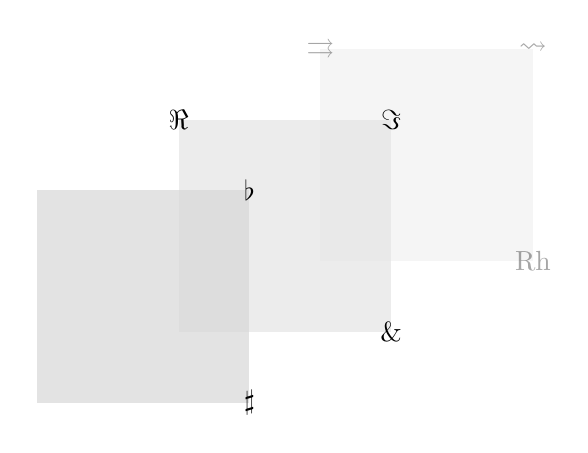
\begin{tikzpicture}[scale=.9]
\begin{scope}[xshift=4cm,yshift=2cm, opacity=.35]
\fill[fill opacity=.75,gray!10] (0,0) rectangle (3,3);
\node (squig) at (0,0) {};
\node (two) at (0,3) {$\rightrightarrows$};
\node (squig2) at (3,3) {$\rightsquigarrow$};
\node (rh) at (3,0) {$\textrm{Rh}$};
\node (fisrt) at ($(squig)!.5!(squig2)$) {$\trhid$};
\end{scope}
\begin{scope}[xshift=2cm,yshift=1cm]
\fill[fill opacity=.75,gray!20] (0,0) rectangle (3,3);
\node (im) at (0,0) {};
\node (re) at (0,3) {$\Re$};
\node (im2) at (3,3) {$\Im$};
\node (and) at (3,0) {$\&$};
\node (fisrt) at ($(im)!.5!(im2)$) {$\secnod$};
\end{scope}
\fill[fill opacity=.75,gray!30] (0,0) rectangle (3,3);
\node (flat) at (0,0) {};
\node (shape) at (0,3) {$\shape$};
\node (flat2) at (3,3) {$\flat$};
\node (sharp) at (3,0) {$\sharp$};
\node (fisrt) at ($(flat)!.5!(flat2)$) {$\fisrt$};
\end{tikzpicture}
\end{center}
\end{frame}
\begin{frame}[label={sec:orgf9c79a3}]{Un esempio workato out: de Rham in coesione}
\end{frame}
\end{document}